\section{Further Work}
Whilst the system produced can be considered a complete system, there are still definitely improvements that could be made, and functionality that could be added. In this section, the main extensions to the system have been detailed, along with their reasoning for not being in the initial release. 

\subsection{Back end Interoperability}
The purpose of the system is to be a web-front end, to a back end that can perform fuzzy inference. This means that the system should not be reliant on back end that it currently uses (FuzzyToolkitUoN), and it could be interchanged with some other back end (potentially with greater functionality, or better performance). This is a result of the system being written almost entirely in JavaScript, making the majority of it's functionality a client-sided affair, and not relying on the back end. The only functionality that the back end truly provides, is the ability to save files to the user's machine, and to evaluate the fuzzy system created. This means that, with the implementation of a simple API layer between the front end and back end, the back end could easily be swapped out to any back end that the user would want. This would allow the user extra functionality within the system, making it much more useful for the expert user. This could include such things as different inference types (like TSK), different t-norms, and t-conorms for the inference methods, and different visualisation techniques. This would make the system much more useful, as it currently can only perform Mamdani inference, with a limited number of inference methods, due to the limited scope of the back end.

\begin{figure}[ht!]
	\begin{center}
		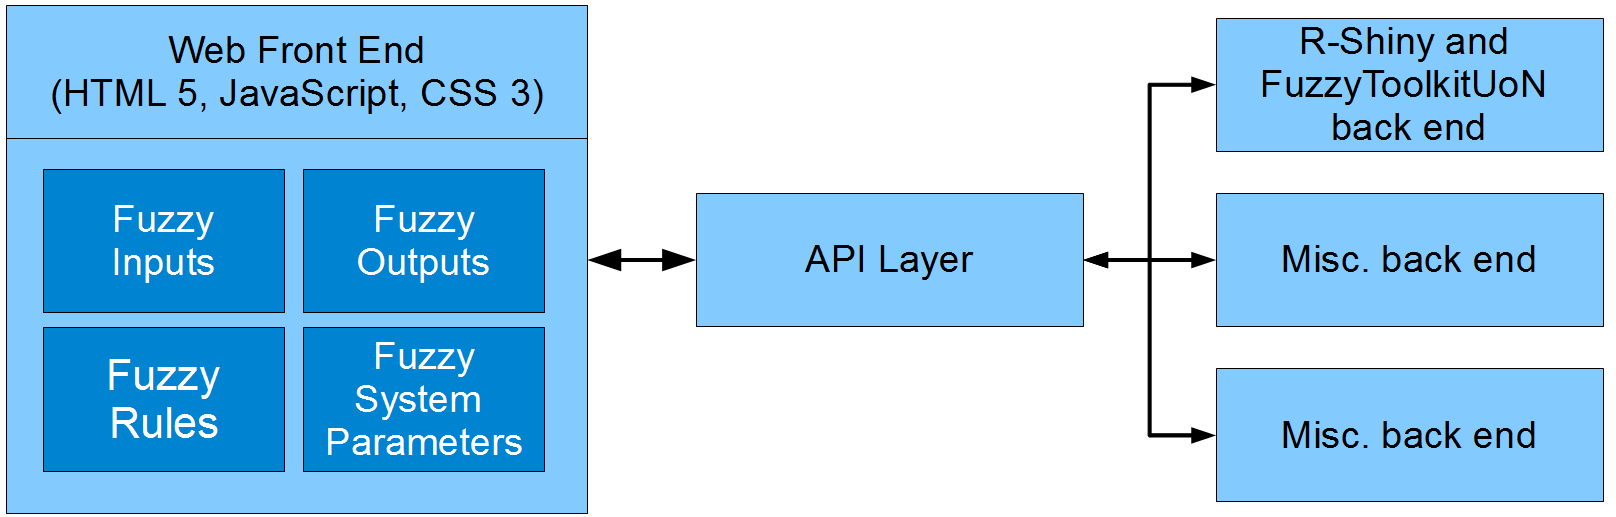
\includegraphics[width=0.9\textwidth]{images/archi-new}
	\end{center}
	\vspace{-2mm}
	\caption{Interaction between the front end of the system and interchangeable back ends}
	\label{fig:fw-interop}
	\vspace{-1mm}
\end{figure}

\subsection{More Usability Improvements}

\subsection{Type-2 Fuzzy Logic Support}
\label{sec:type2}
The purpose of a type-1 fuzzy logic system, is to model uncertainty in the terms that humans use to describe properties. Unfortunately, this raises a paradox; fuzzy sets have a connotation of uncertainty, but the membership functions used are entirely certain once their parameters have been specified \cite{mendel2003type}. Type-2 fuzzy logic attempts to rectify this paradox, in the sense that uncertainty is not only limited to the terms used, but also the membership functions defined \cite{castillo2003type}. This means that each membership function defined has a third dimension, which allows an additional degree of freedom, to directly modal uncertainty \cite{mendel2002type}.

\begin{figure}[ht!]
	\begin{center}
		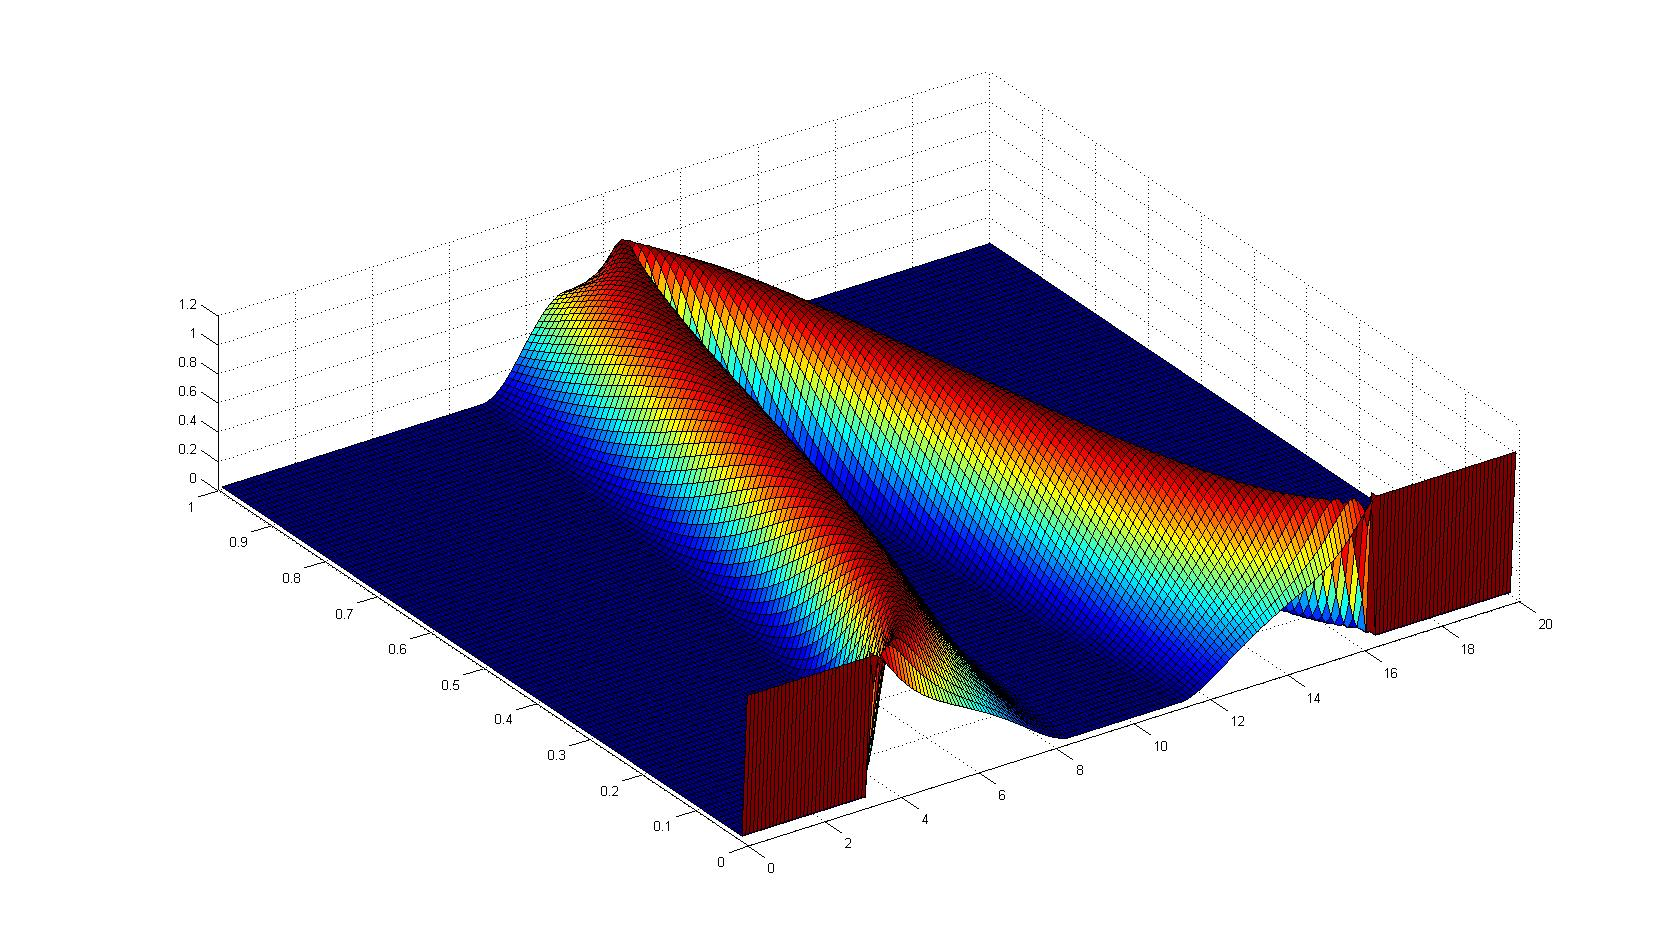
\includegraphics[width=0.5\textwidth]{images/type2set}
	\end{center}
	\vspace{-4mm}
	\caption{An example type-2 fuzzy set}
	\label{fig:fw-type2}
	\vspace{-1mm}
\end{figure}

As mentioned in the introduction to this report, type-2 fuzzy logic is not supported in this software. This is because the jump in knowledge between type-1 fuzzy logic (that \emph{is} supported), and type-2, is extremely large, and would not be suitable for novice users. Other reasons include a lack of time to implement such a large feature, and that type-2 fuzzy logic is still not widely adopted in the field. If more time was allocated to the project, this could have been implemented along side the type-1 system, however an entirely new back end would have been needed, as the current back end, FuzzyToolkitUoN, does not support type-2 fuzzy logic. Adding type-2 support to the system would have greatly improved it's usefulness and practicality, and could have easily made the tool a niche within the market, and the preferred software to use among experts. This would have been due to the ease of access, and ease of use of the system, which are  features that most type-2 software systems currently available are lacking (such as Juzzy \cite{wagner2013juzzy}, which requires an installation of Java before it can be used).

\subsection{Customisations}
The ability to customise a website has been identified as one of the key factors for website success \cite{fan2010factors}. It has been found that the user's are more likely to return to a piece of software, if it is customised to their needs, and thus more personal. Unfortunately, there are not many customisations that could be made with this system, but some could be implemented to help improve user experience. One of these could be the look and feel of the system, which is currently a minimalistic white design. Some users prefer to use a darker interface (especially when completing work in the evening), and thus a set of different colour schemes could be employed, which would both serve a practical purpose, and an aesthetic one. Another potential customisation could be the ability to switch to an ``expert'' mode, where help is less present in the system, more keyboard short cuts are supported, and there is less GUI to navigate. This would greatly increase the speed in which an expert user could complete their task within the system, as there would be less distractions.